\section{Soběpodobnost}\label{sec:sobepodobnost}
Mandelbrot si uvědomil, že struktura pobřeží se charakterově vymyká útvarům do tehdy známým eukleidovské geometrii, neboť mapy s různými měřítky poskytovaly různou úroveň detailů, které hrály netriviální roli v jeho celkové délce. Učinil však jiné zásadní pozorování, a to sice, že mnoho detailů má společné rysy, které se opakují. Hodně z nich se shodovalo s výjimkou jejich měřítka. \citep[str. 96]{Mandelbrot1983}\par

Ve fraktální geometrii se pro tento úkaz uchytil termín \emph{soběpodobnost} (angl. \emph{self-similarity}). Útvar nazýváme soběpodobným, \textbf{pokud se sám sobě podobná v libovolném měřítku} \citep[str. 220]{Voracova2022} nebo pokud \textbf{část útvaru je podobná jeho celku}. Zmíněná podoba může být míněna přibližně (např. v případě pobřeží je nejspíše jasné, že žádné z jeho detailů nesdílejí společné rysy přesně), ale v dalších částech si předvedeme soběpodobnost \emph{přímou}.

\subsection{Kochova křivka}\label{subsec:kochova_krivka}
Na začátku vezmeme úsečku délky $1$. Vyjmeme prostřední (tj. druhou) třetinu a nahradíme ji úsečkami délky $1/3$, tak, aby na sebe navazovaly v krajních bodech. Tento proces následně opakujeme pro nově vzniklé úsečky. Obecně u úsečky délky $l$ nahradíme její prostřední třetinu dvojicí úseček délek $l/3$ (viz obrázek \ref{fig:kochova_krivka_6iteraci}).
\begin{figure}[h]
    \centering
    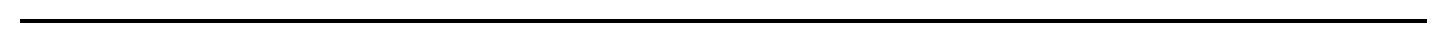
\includegraphics[scale=\fractalscale]{ch01_kochova_krivka_0iterace.pdf}\qquad
    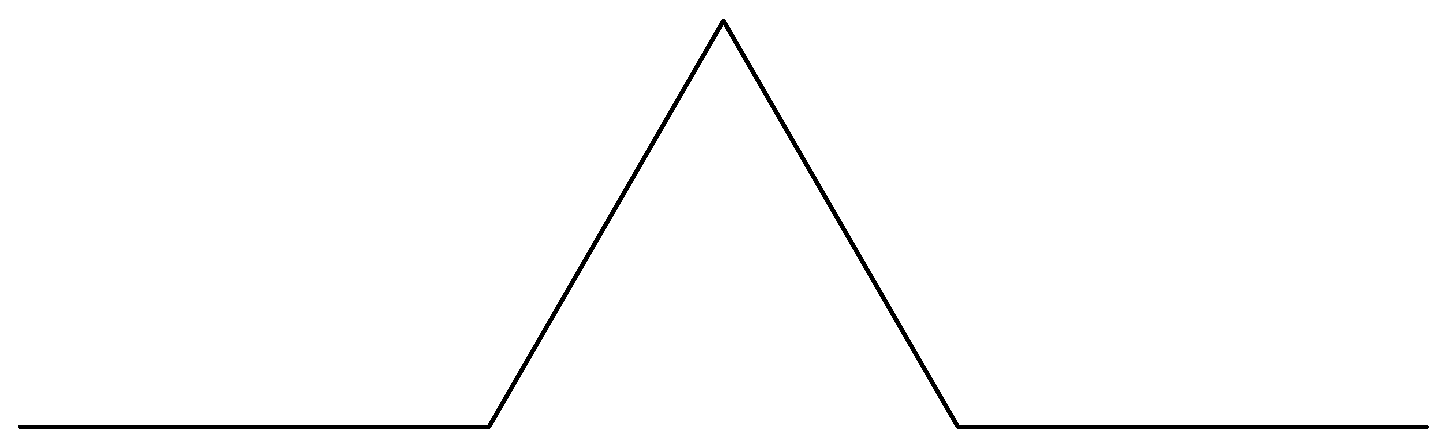
\includegraphics[scale=\fractalscale]{ch01_kochova_krivka_1iterace.pdf}\qquad
    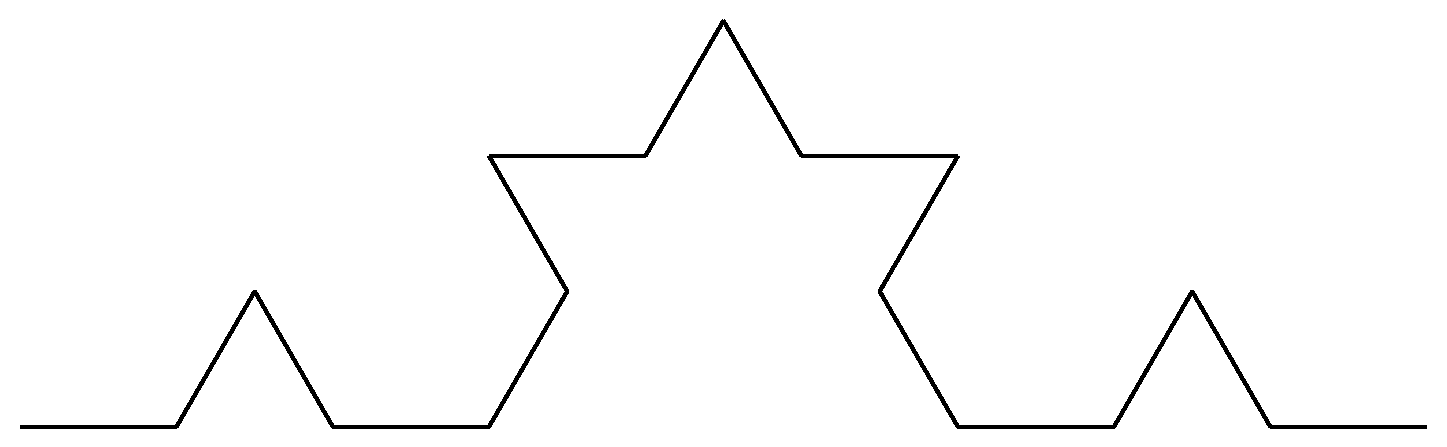
\includegraphics[scale=\fractalscale]{ch01_kochova_krivka_2iterace.pdf}\qquad
    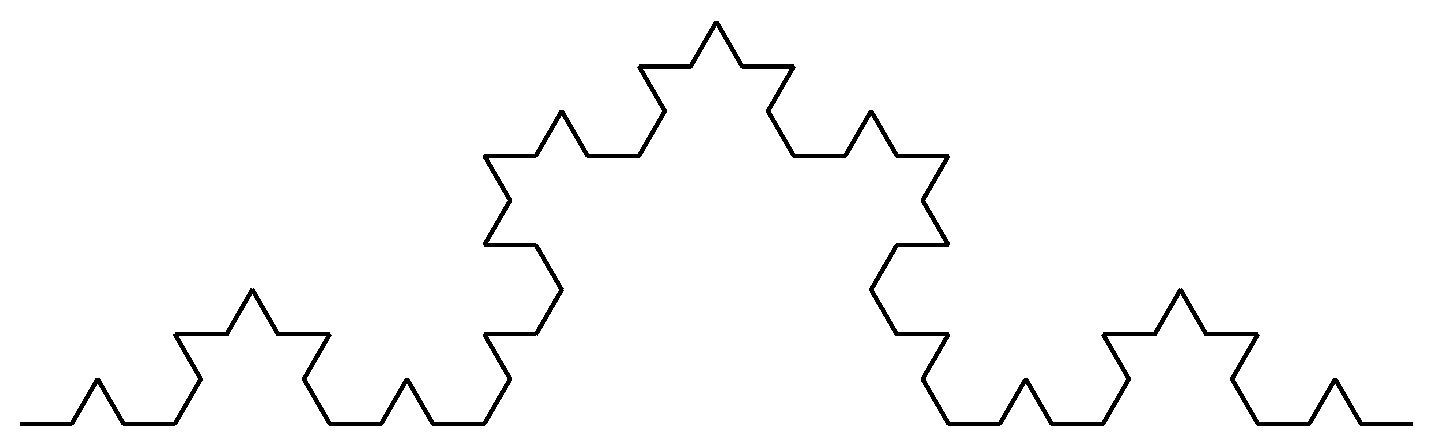
\includegraphics[scale=\fractalscale]{ch01_kochova_krivka_3iterace.pdf}\qquad
    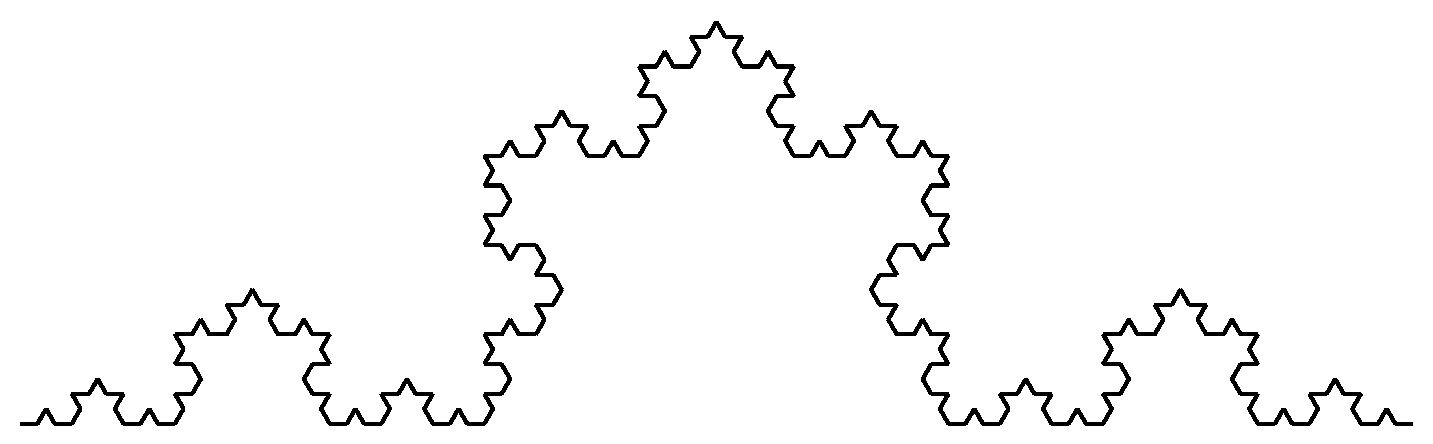
\includegraphics[scale=\fractalscale]{ch01_kochova_krivka_4iterace.pdf}\qquad
    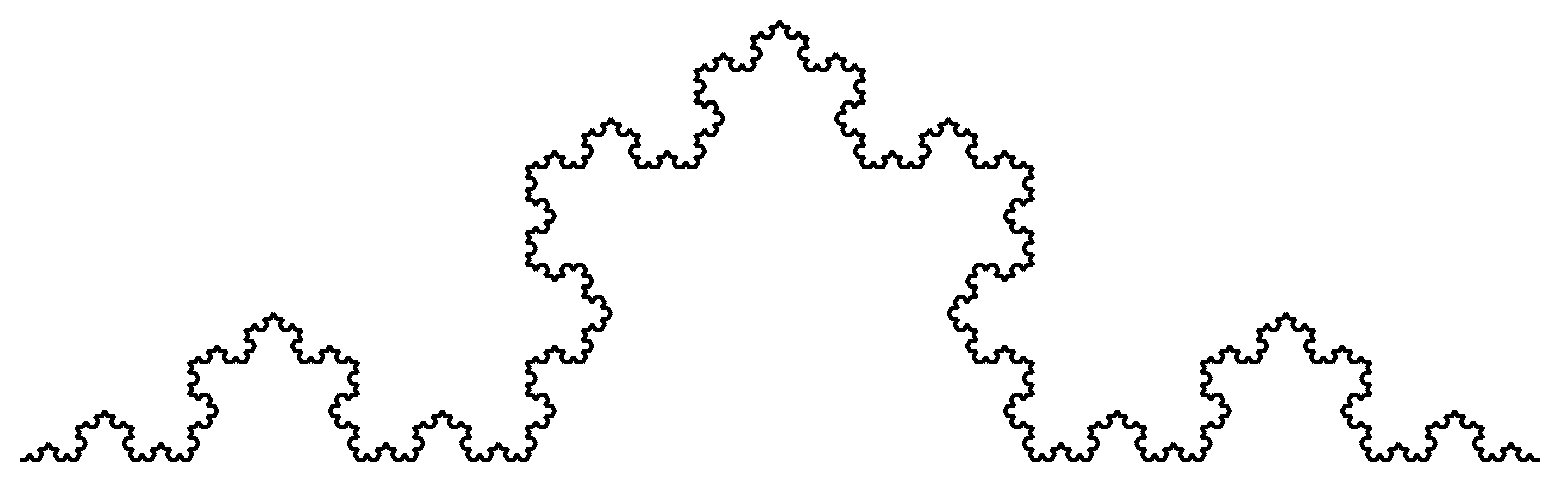
\includegraphics[scale=\fractalscale]{ch01_kochova_krivka_5iterace.pdf}
    \caption{Prvních šest iterací Kochovy křivky.}
    \label{fig:kochova_krivka_6iteraci}
\end{figure}
V první řadě si můžeme všimnout, že v každé další iteraci jsou nově vzniklé podobné původnímu celku, tedy v předešlé iteraci (viz obrázek \ref{kochova_krivka_podobnost}). Pokud by tento proces pokračoval do nekonečna, pak by každá ze čtyř částí křivky představovala \textbf{celý původní obrazec} ve zmenšeném měřítku (byla by tedy soběpodobná).
\begin{figure}[h]
    \centering
    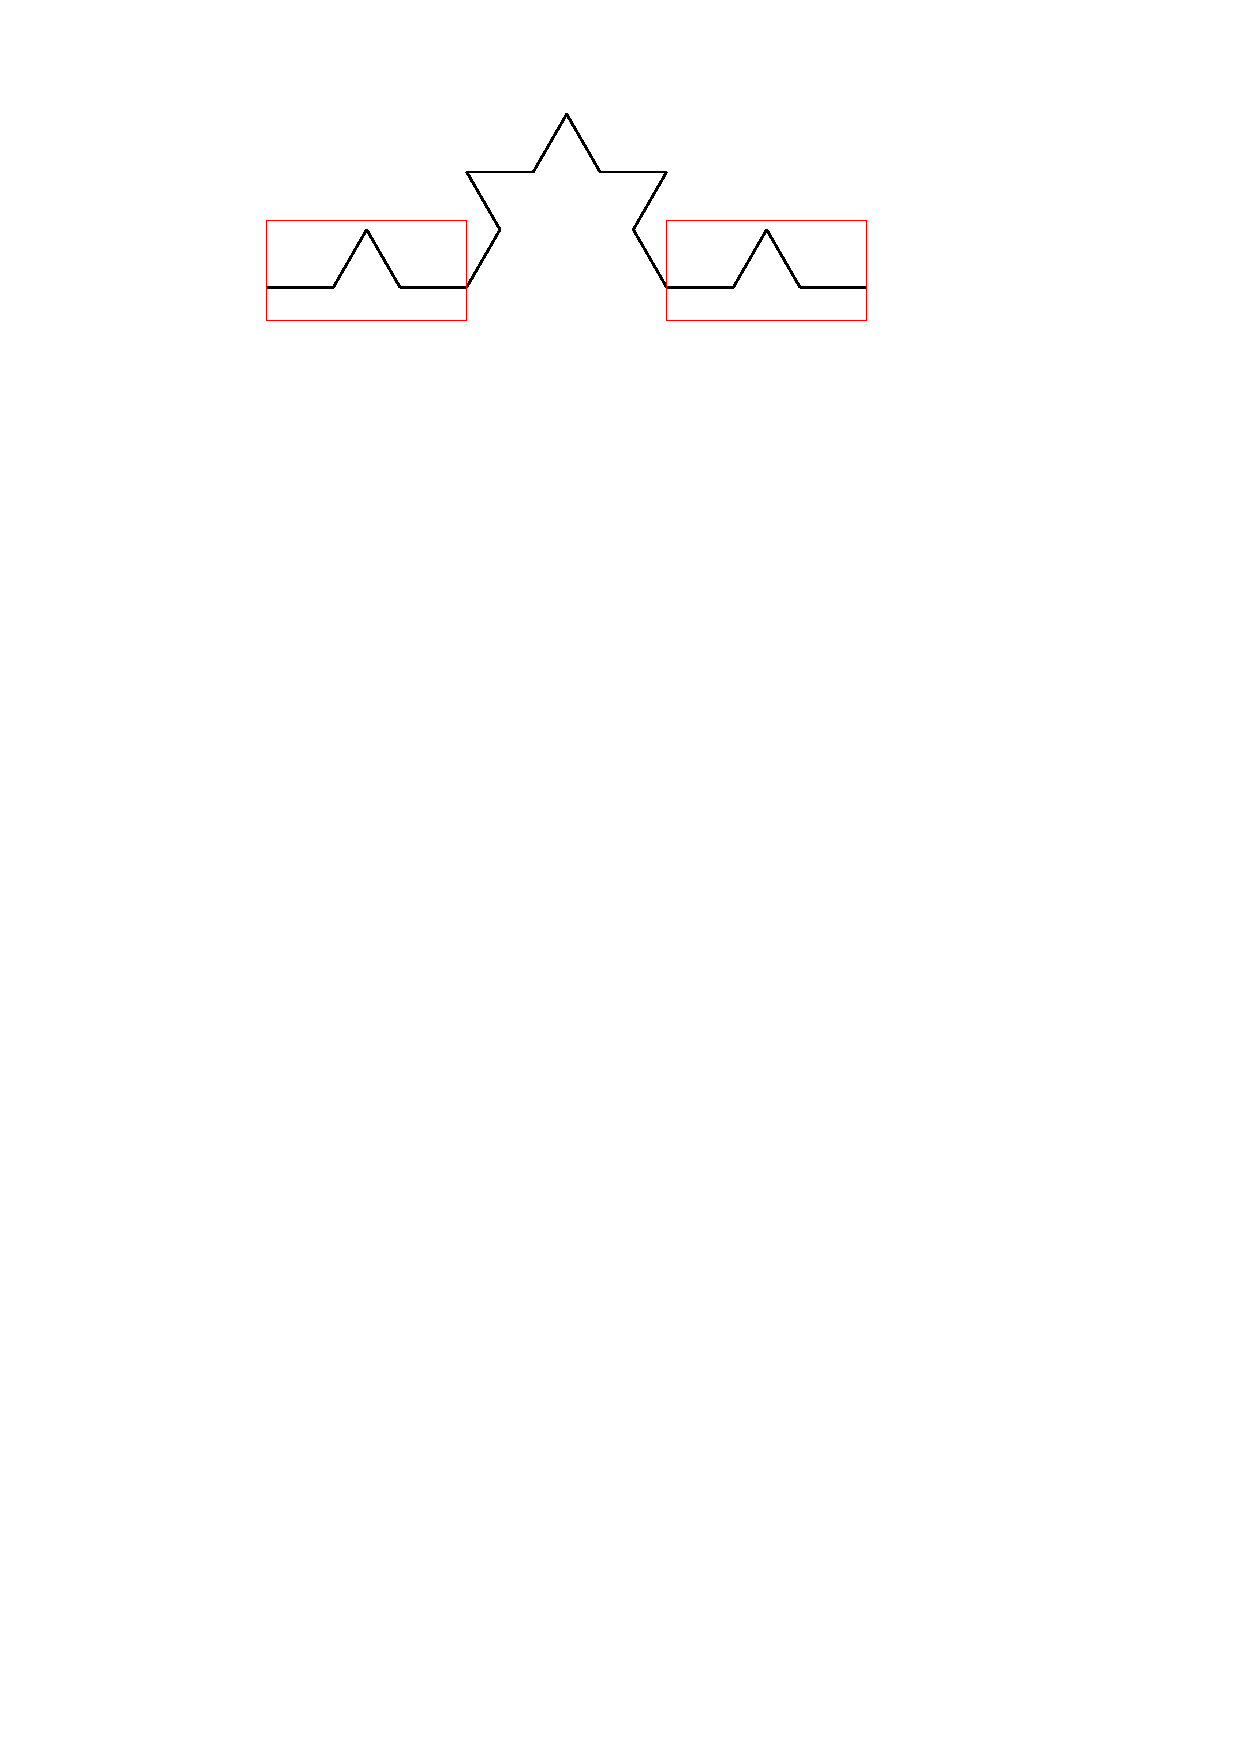
\includegraphics[scale=\normalipe]{ch01_kochova_krivka_podobnost.pdf}
    \caption{Druhá iterace Kochovy křivky "uvnitř" třetí v menším měřítku.}
    \label{fig:kochova_krivka_podobnost}
\end{figure}
Zkusme se nyní podívat na délku křivky. V první iteraci začínáme s úsečkou délky\footnote{Mohli bychom také začít s obecnou délkou $l_0$, ale ta by se však při výpočtu projevila pouze jako konstantní násobek.} $1$, která se v druhé iteraci změní na křivku délky $4/3$. Není těžké si rozmyslet, že obecně v $n$-té iteraci bude délka křivky $l_n$ rovna
\begin{equation*}
    \left(\dfrac{4}{3}\right)^{n-1}.
\end{equation*}
Posloupnost $\{l_n\}_{n=1}^{\infty}$ je geometrická s kvocientem $4/3>1$, a tedy její limita je $\infty$. Kochova křivka má tedy nekonečnou délku.